\documentclass[t,14pt,aspectratio=169]{beamer}
\usepackage{ep-dark}   % JHU/WSE style for use on Lightboard
\usepackage{graphicx}  % for inclusion of graphics
\usepackage{amsmath}   % good for additional math
\usepackage{amsthm}    % theorems, definitions, etc
%\usetheme{CambridgeUS}

%% This is the UT logo in the top right.
%% -------------------------------------
\usepackage{tikz}
\logo { 
\begin{tikzpicture}[overlay,remember picture]
\coordinate (A) at (-2.0,7.7);
\node[left=0.2cm] at (current page.27){
    %
\includegraphics[width=3cm]{Figures/General/UT_WBMW_Rot_RGB_01.png}
    
\includegraphics[width=3cm]{Figures/General/UT_WBMW_Weiss_1C_tr.png}    
};
\node[text=Karminrot] at (A) {\tiny Introduction to Geophysics};
\end{tikzpicture}
}
%% -------------------------------------



\title{Introduction to Geophysics}
\author{R. Drews}
\date{\today}


\begin{document}

% These commands create the first slide
% \coursename specifies the name of the course. No need to include the
% course number especially since they change from time to time
%
% \modulename is the name of this particular lesson

\coursename{Introduction to Geophysics}
\modulename{Gravimetry}
\titleframe
\begin{frame}
  \frametitle{Some title}
  \setlength{\leftmargini}{0.5em}
  \begin{columns}[c, onlytextwidth]%EVEN SPECIFYING THE c OPTION
      \begin{column}{.6\textwidth}%
          \setlength{\partopsep}{0pt}%AND EVEN REMOVING EXTRA itemize SPACE
          % Keep this empty
      \end{column}%
      \begin{column}{.35\textwidth}

          %\includegraphics[width=\textwidth]{example-image}
          %\tiny [Source]
          \alert{Learning Goals:}
          \begin{center}
          \begin{itemize}
            \itemsep 1.0em
                \item First item bla bla bla bla some more text
                \item First item bla bla bla bla some more text
                \item First item bla bla bla bla some more text
            \end{itemize}
      \end{center}
      \end{column}%
  \end{columns}
  \end{frame}




\begin{frame}
  \frametitle{Gravitational field}
  \begin{columns}[onlytextwidth] 
    \begin{column}{.6\textwidth}
      \centering
      asdf
      %Leave this space empty for the lightboard person to stand.
    \end{column}%
    \hfill%
    \begin{column}{.4\textwidth}
     
    This is above
      \begin{itemize}
        \itemsep 0.8em
        \item point 1
        \item point 2
    
      \end{itemize}
 
    This is below
 
    \end{column}%
    \end{columns}
\end{frame}

\begin{frame}
  \frametitle{Beamer}
  \large

  We use \alert{Beamer} instead of PowerPoint to create presentations
  to be projected on a screen. Since it is based on \LaTeX, it is
  excellent for presentations with mathematical formulas.

  Indeed, we assume the user is already familiar with \LaTeX.
\end{frame}

\begin{frame}
  \large

  This slide deck uses the \texttt{ep-dark} style which provides a
  particularly simple, clean design featuring white text on a black
  backgound. This is ideal for use on the Lightboard.

  Keep it clean! Don't put too many words on a slide.
\end{frame}


\begin{frame}
  \frametitle{Blocks}
  \large
  \begin{block}{This is a block}
    A \alert{block} structure is useful for highlighting particular
    information.
  \end{block}

  \begin{definition}
    The \alert{definition} environment is a type of block used for
    definitions. Highlight the word you are defining.
  \end{definition}
\end{frame}

\begin{frame}
  \frametitle{Itemized lists}
  \large
  \begin{itemize}
  \item<+-> Itemized lists are useful for sequential points.
  \item<+-> In this example, each item appears on subsequent slides.
  \item<+-> Items are added one by one until done. 
  \end{itemize}
\end{frame}

\begin{frame}
  \frametitle{Pauses}
  \Large The \alert{pause} command 
  \pause 
  is a mechanism for building up a slide in pieces.
\end{frame}


\begin{frame}
  \frametitle{Only}
  \large  

  The \alert{only} command provides more fine control in revealing
  material on a slide.

  \only<2>{
    This sentence will only appear after the first the first one.
  }

  \only<3->{
    The second sentence was only on the $2^{\text{nd}}$ slide; this
    sentence will be on slides 3 and all subsequent slides.
  }

  \only<4>{
    Finally, this sentence appears.
  }

\end{frame}

\begin{frame}
  \frametitle{Mathematics}
  \large
  Because Beamer is built in \LaTeX\ it does mathematics beautifully
  either inside a sentence, $\sqrt2 + \cos\theta$, or in display mode:
  \[
  x = \frac{-b \pm \sqrt{b^2-4ac}}{2a} .
  \]

  Do it right! Notice this difference between $cos\theta$ [wrong!] and
  $\cos\theta$ [yes!]. 
\end{frame}

\begin{frame}
  \frametitle{Aligned equations}
  \large The \alert{aligned} environment (in math mode) works well
  with Beamer and pauses:
  \[
  \begin{aligned}
    |z| &= \sqrt{z \cdot \overline{z}} \\[12pt]
    \pause
    \therefore |a+bi| &= \sqrt{(a+bi)(a-bi)} \\ \pause
    &= \sqrt{a^2 +abi -abi - b^2i^2} \\ \pause
    &= \sqrt{a^2 + b^2}
  \end{aligned}
  \]
\end{frame}

% \begin{frame}
%   \frametitle{Figures}
%   \large 
%   The \alert{graphicx} package provides the \alert{includegraphics}
%   command. Prepare graphics with a drawing program using light colored
%   lines and shapes on a black or transparent background. Save in a
%   standard graphics format.
%   \begin{center}
%     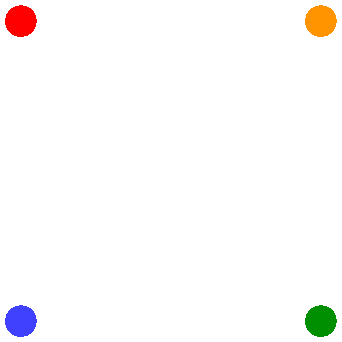
\includegraphics[scale=0.5]{figure}
%   \end{center}
% \end{frame}

\begin{frame}
  \frametitle{Math extras}
  \large
  Use the \alert{amsmath} and \alert{amsthm} packages for additional
  math functionality.

  \begin{theorem}[Binomial]
    Let $n$ be a nonnegative integer. Then
    \[
    (x+y)^n = \sum_{k=0}^n \binom{n}{k} x^k y^{n-k}. \qed
    \]
  \end{theorem}
\end{frame}


\end{document}
